% výběr
Na internetu se dá najít spoustu cloudových řešení, které bych mohl využít. Já jsem zvolil platformu \gls{firebase} od 
Googlu. Upřednostnil jsem ji před jinými řešeními, z nichž některá byla přímo vytvořená pro sběr a zobrazení dat 
z chytrých senzorů. Důvodů bylo několik. Řešení vytvořená \uv{na míru} měla zásadní problém v tom, že většinou v tarifu 
zdarma měla nějaké významné omezení, například omezení ukládaných dat pouze na poslední tři měsíce a platit se mi 
nechtělo. Z ostatních jsem vybral právě \gls{firebase}, poněvadž měl rozumně nastavené limity zdarma, nádhernou 
dokumentaci a zároveň za ním stojí velká firma, takže se nemusím bát, že za rok skončí.

% založení
\gls{firebase} je služba Googlu, takže jediné co je potřeba pro založení je Google účet, díky tarifu zdarma ani nechce 
žádnou platební kartu. Založení projektu se pokusím osvětlit několika obrázky. Počáteční adresa je 
\url{https://console.firebase.google.com/u/0/}

% krok 1
\begin{figure}[H]
    \centering
    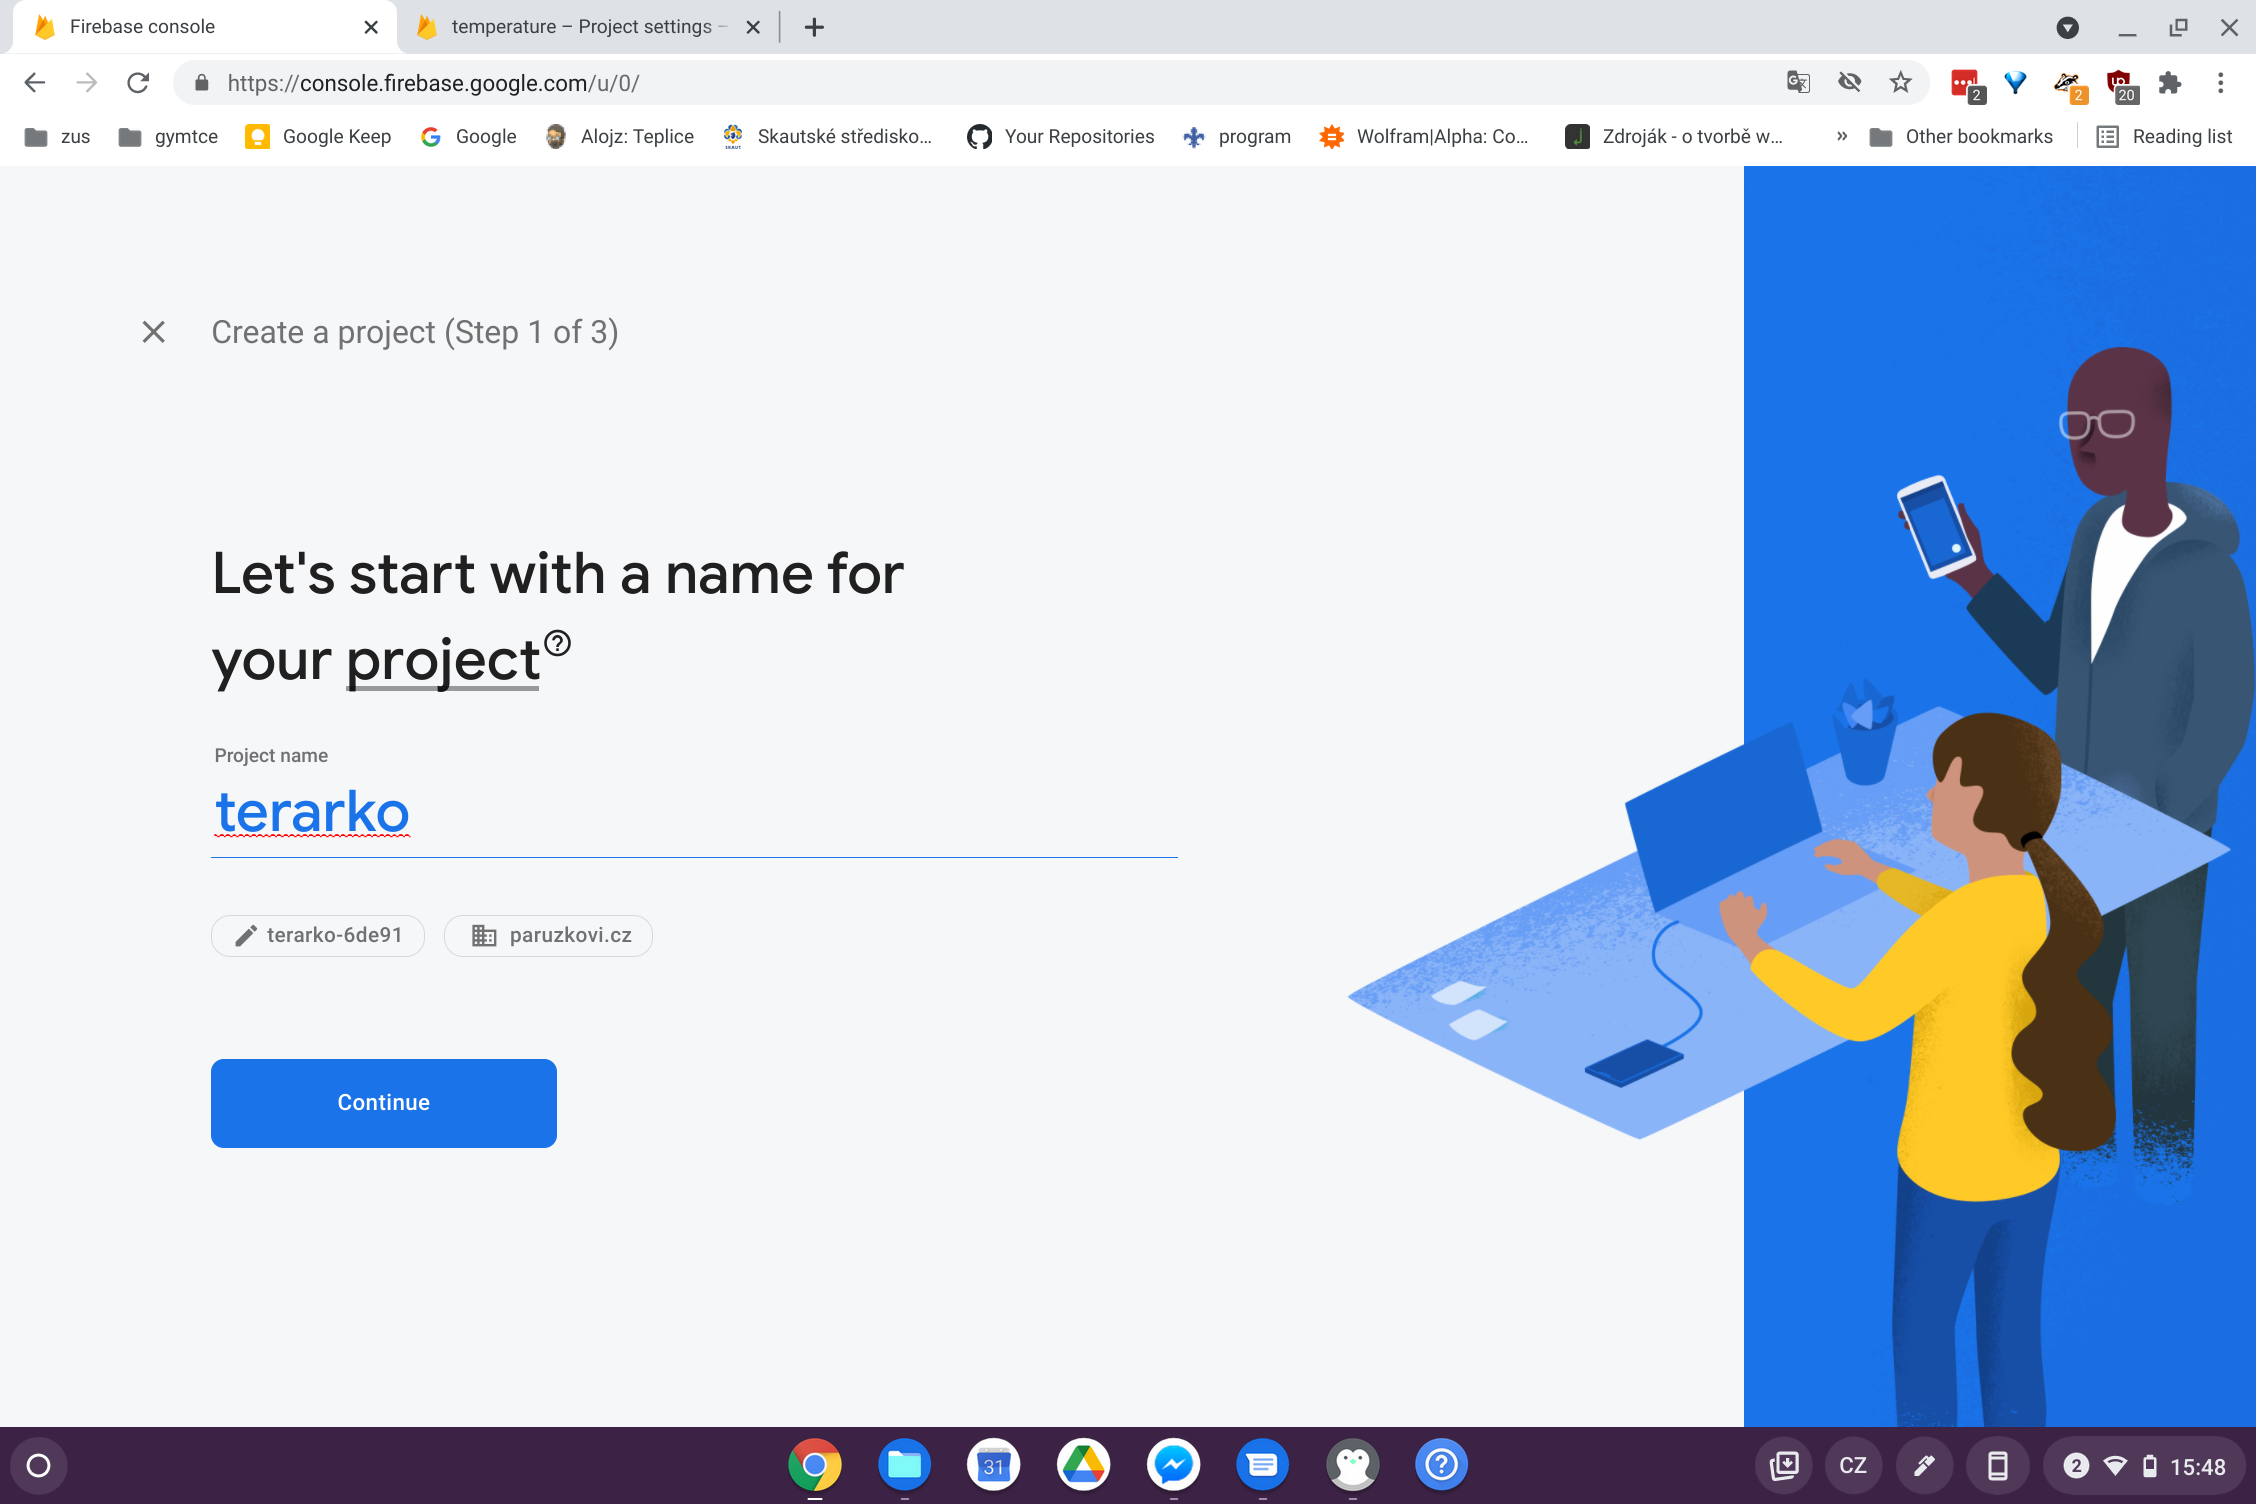
\includegraphics[width=0.8\textwidth]{firebase-1.png}
    \caption{Firebase, krok 1}
\end{figure}
V kroku 1 vybírám projektu jméno.
%krok 2
\begin{figure}[H]
    \centering
    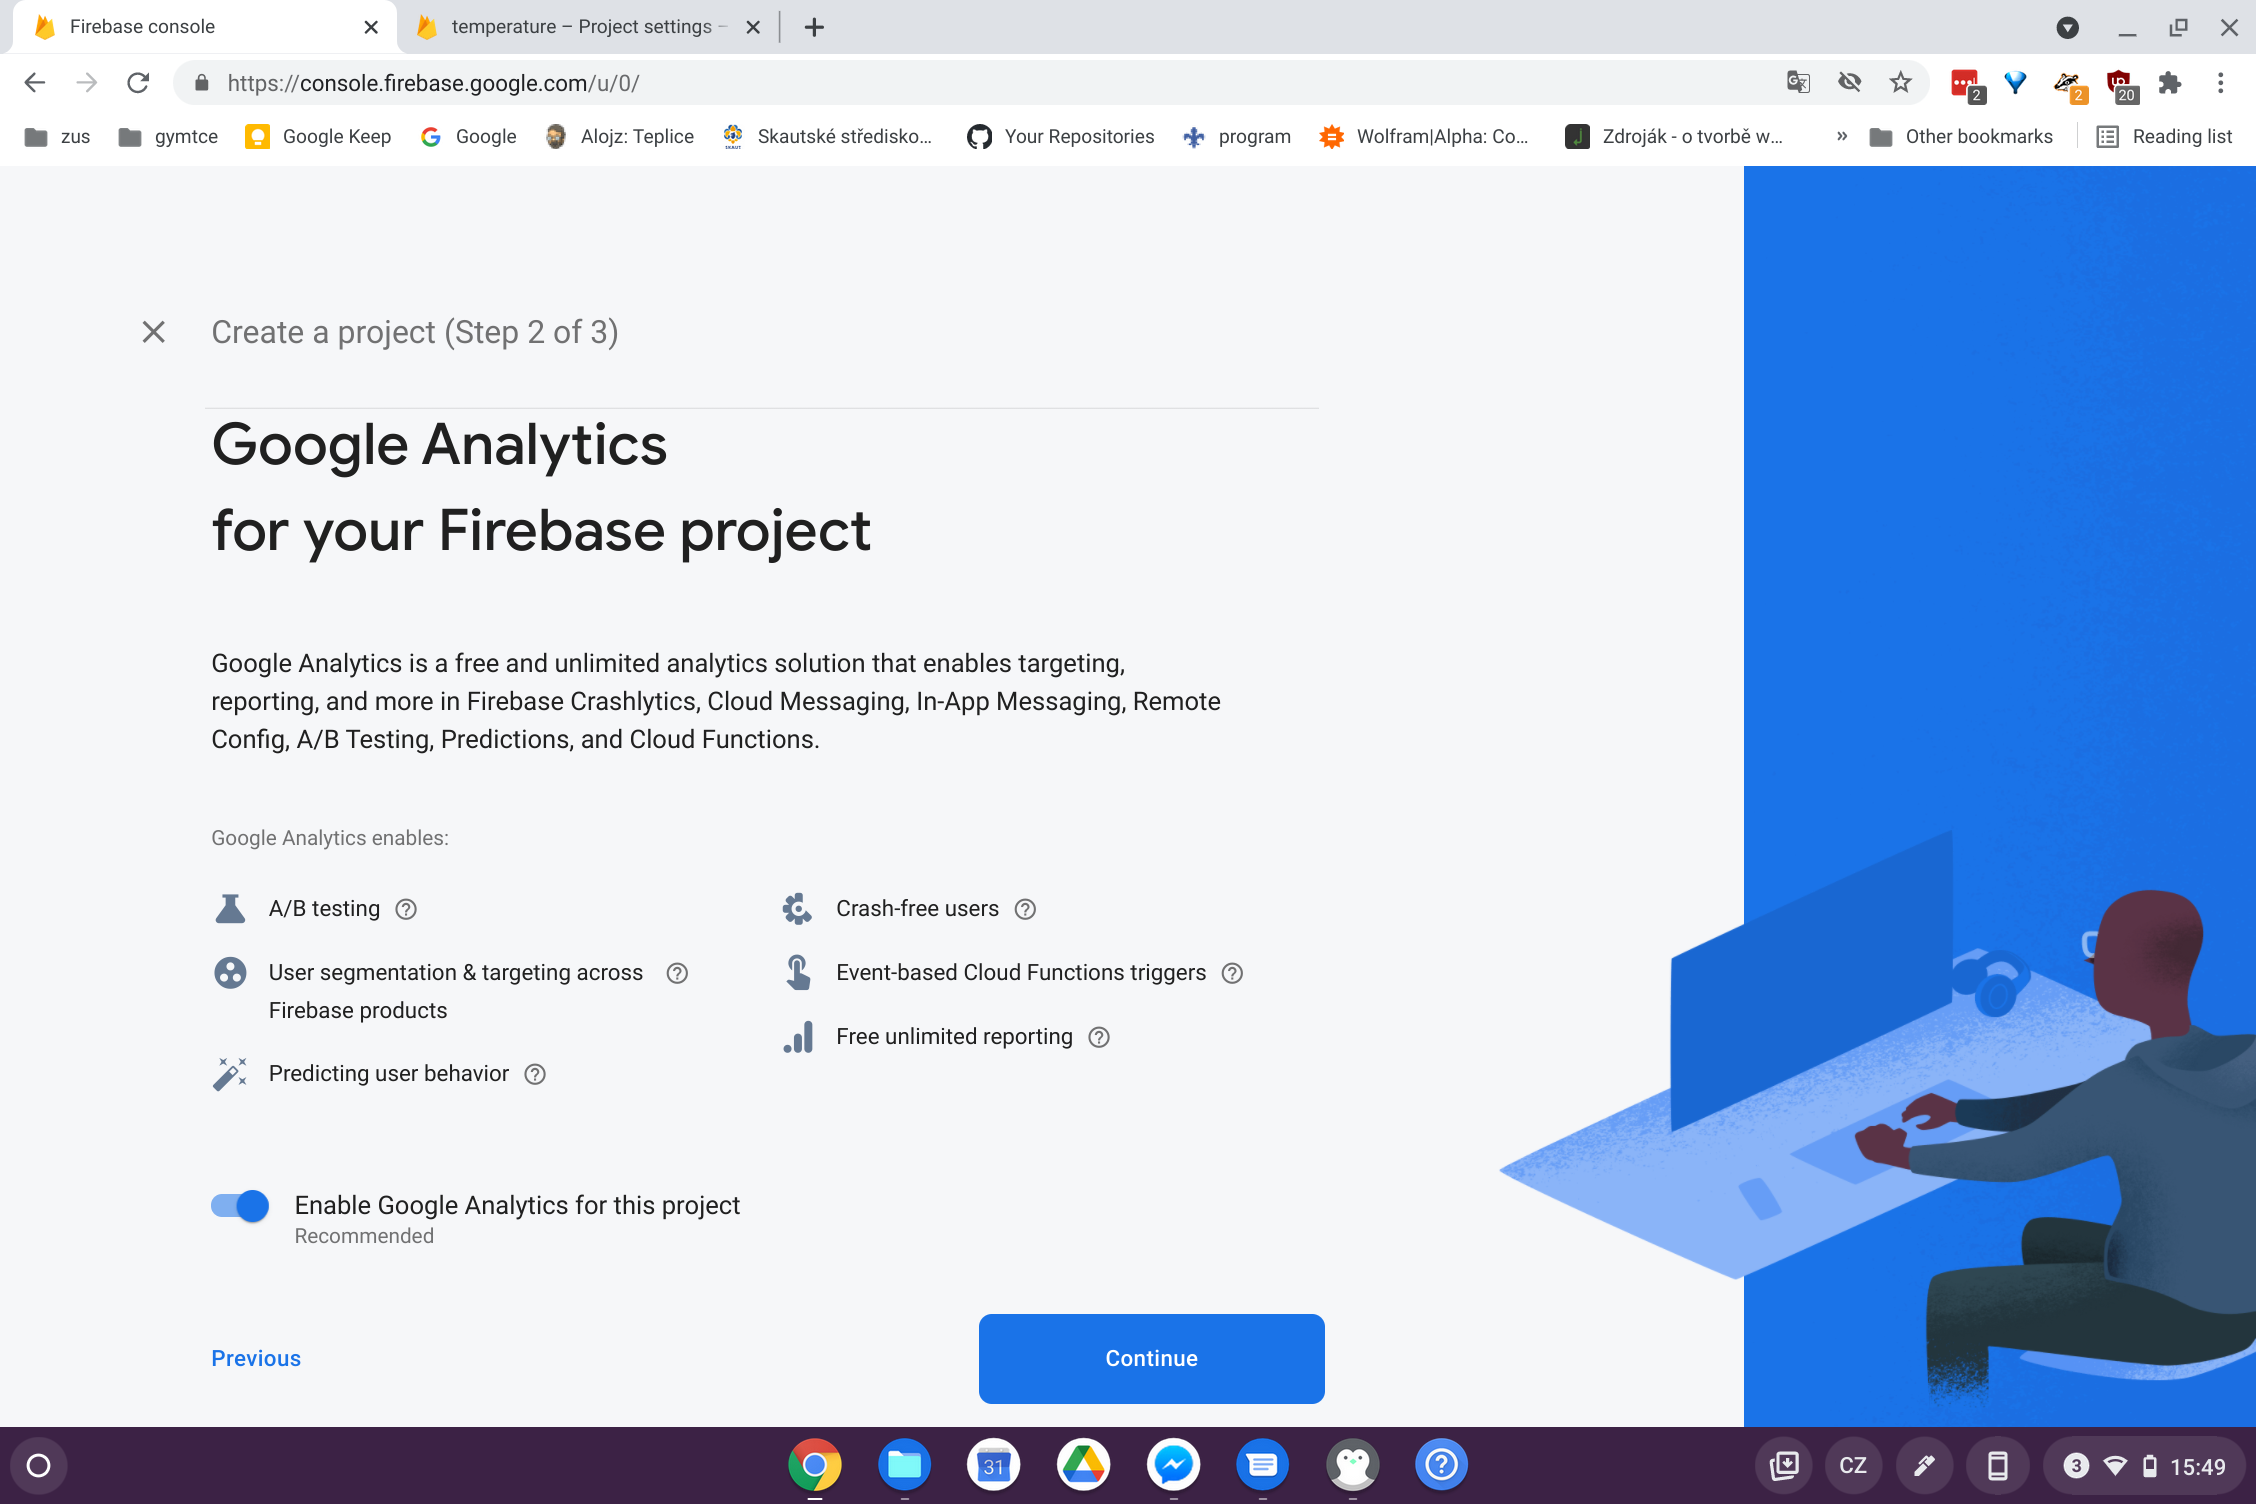
\includegraphics[width=0.8\textwidth]{firebase-2.png}
    \caption{Firebase, krok 2}
\end{figure}
V kroku 2 můžu pro projekt povolit Google Analytics.
% krok 3
\begin{figure}[H]
    \centering
    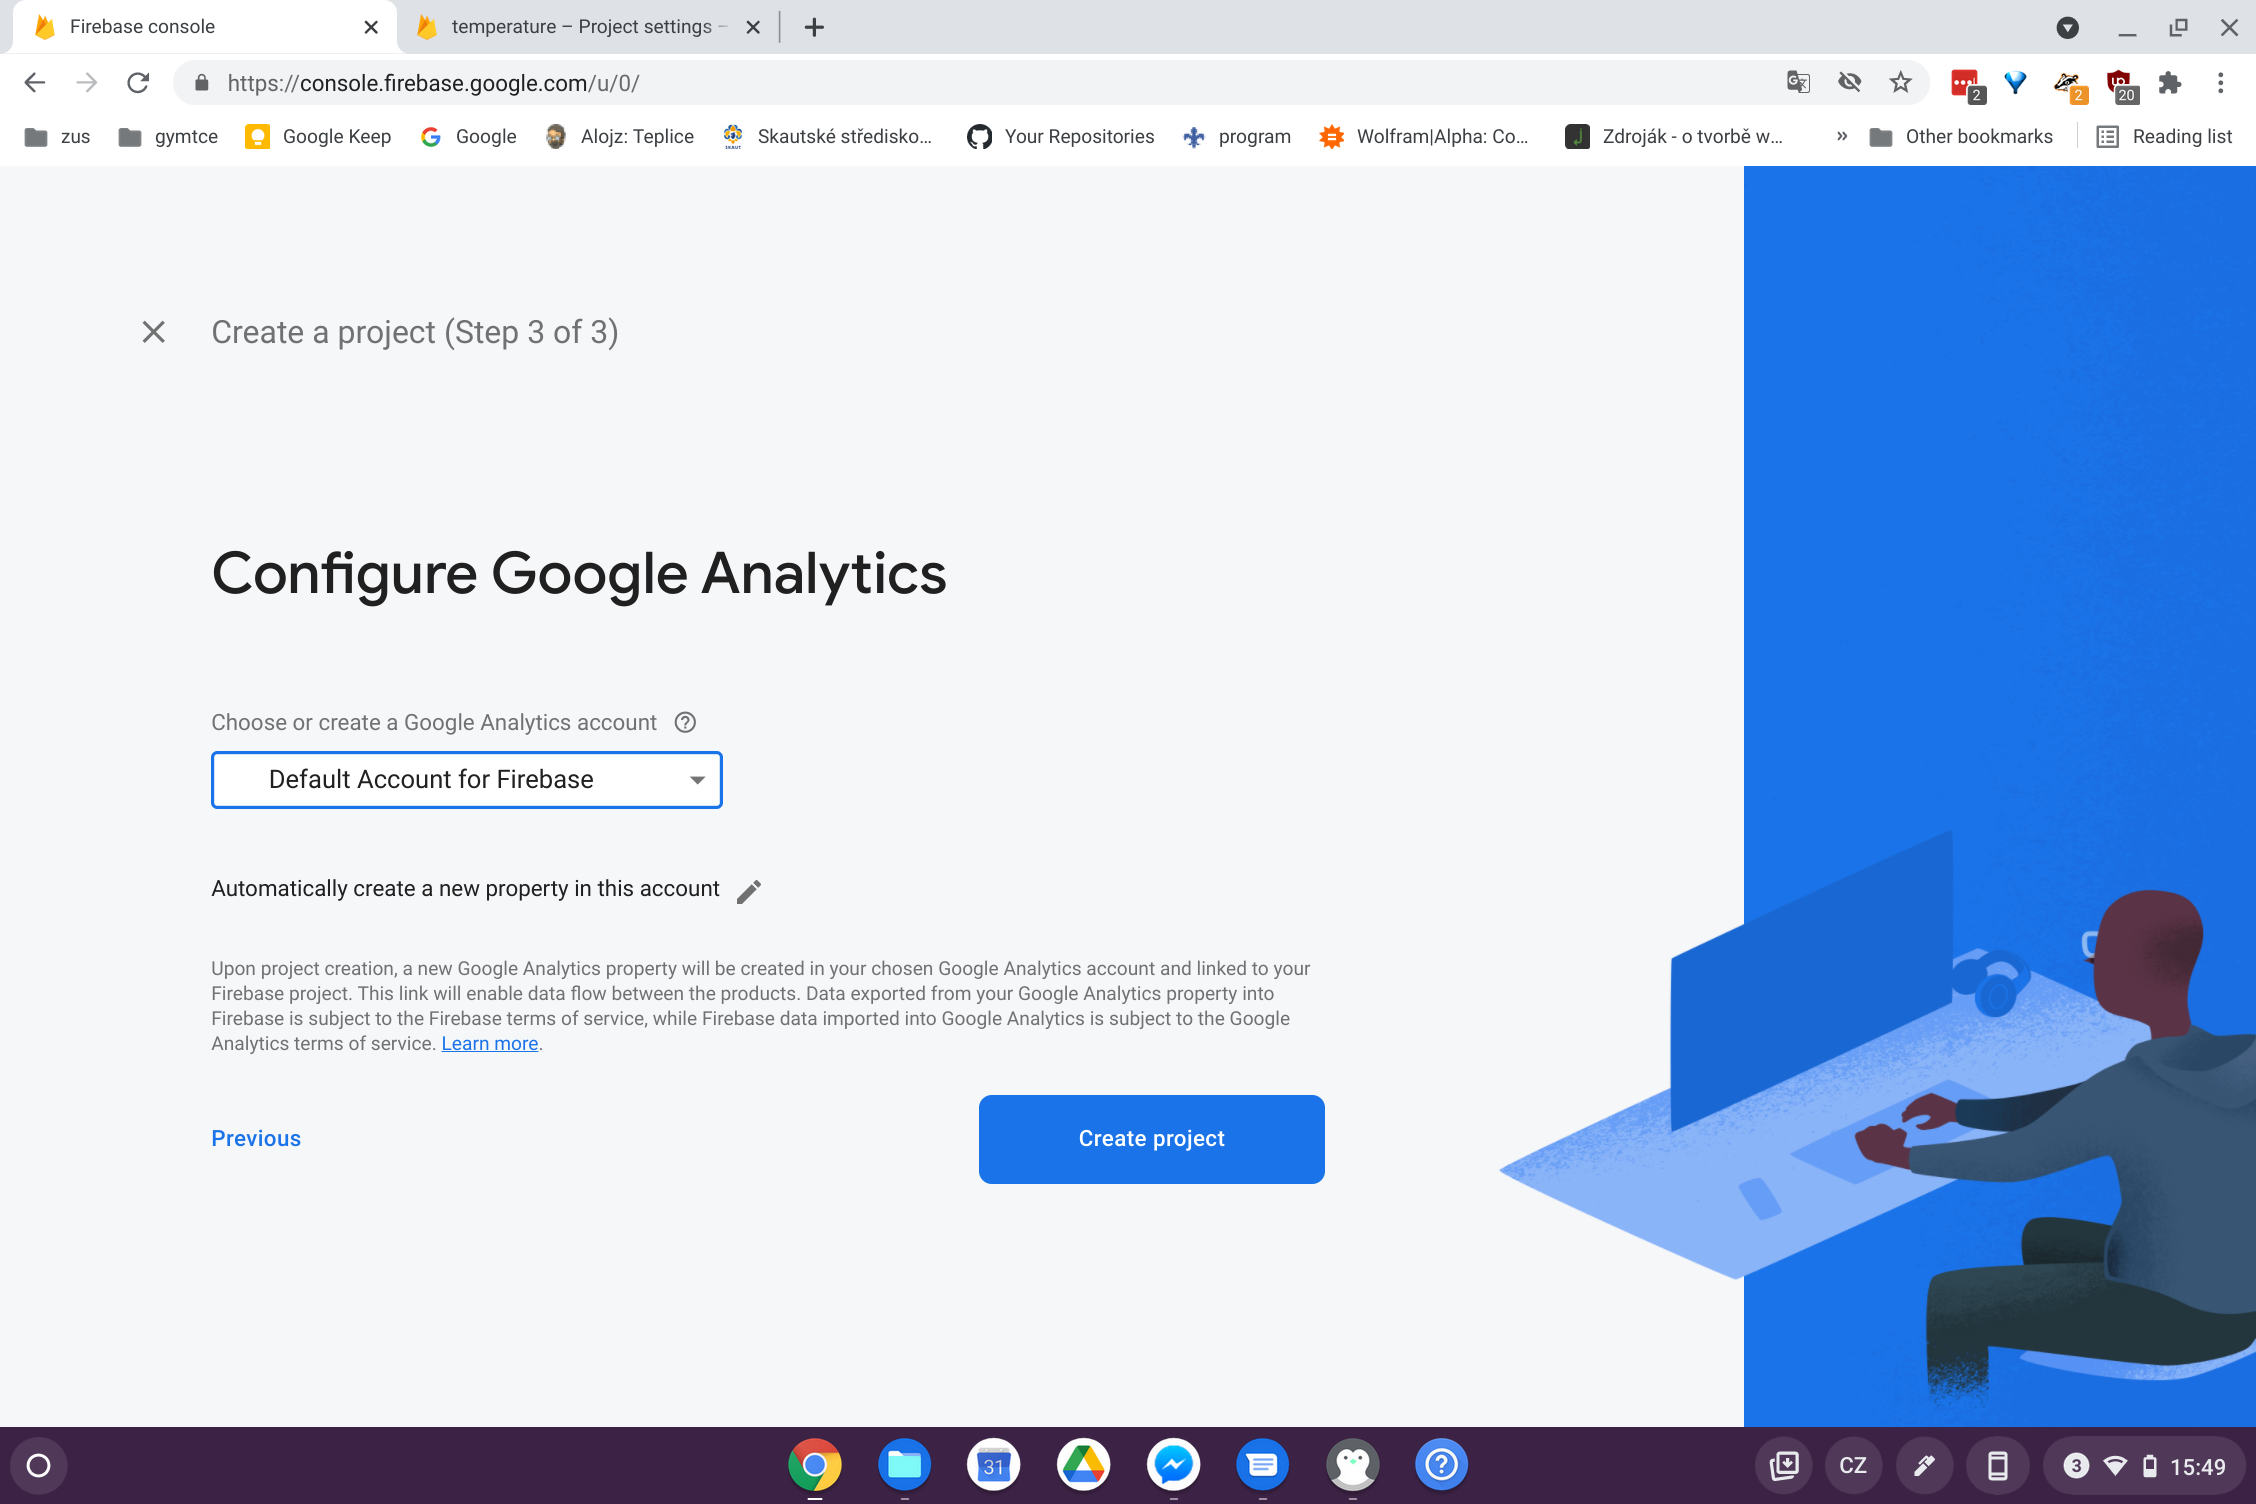
\includegraphics[width=0.8\textwidth]{firebase-3.png}
    \caption{Firebase, krok 3}
\end{figure}
V kroku 3 přiřazuji účet Google Analytics.% hotovo
\begin{figure}[H]
    \centering
    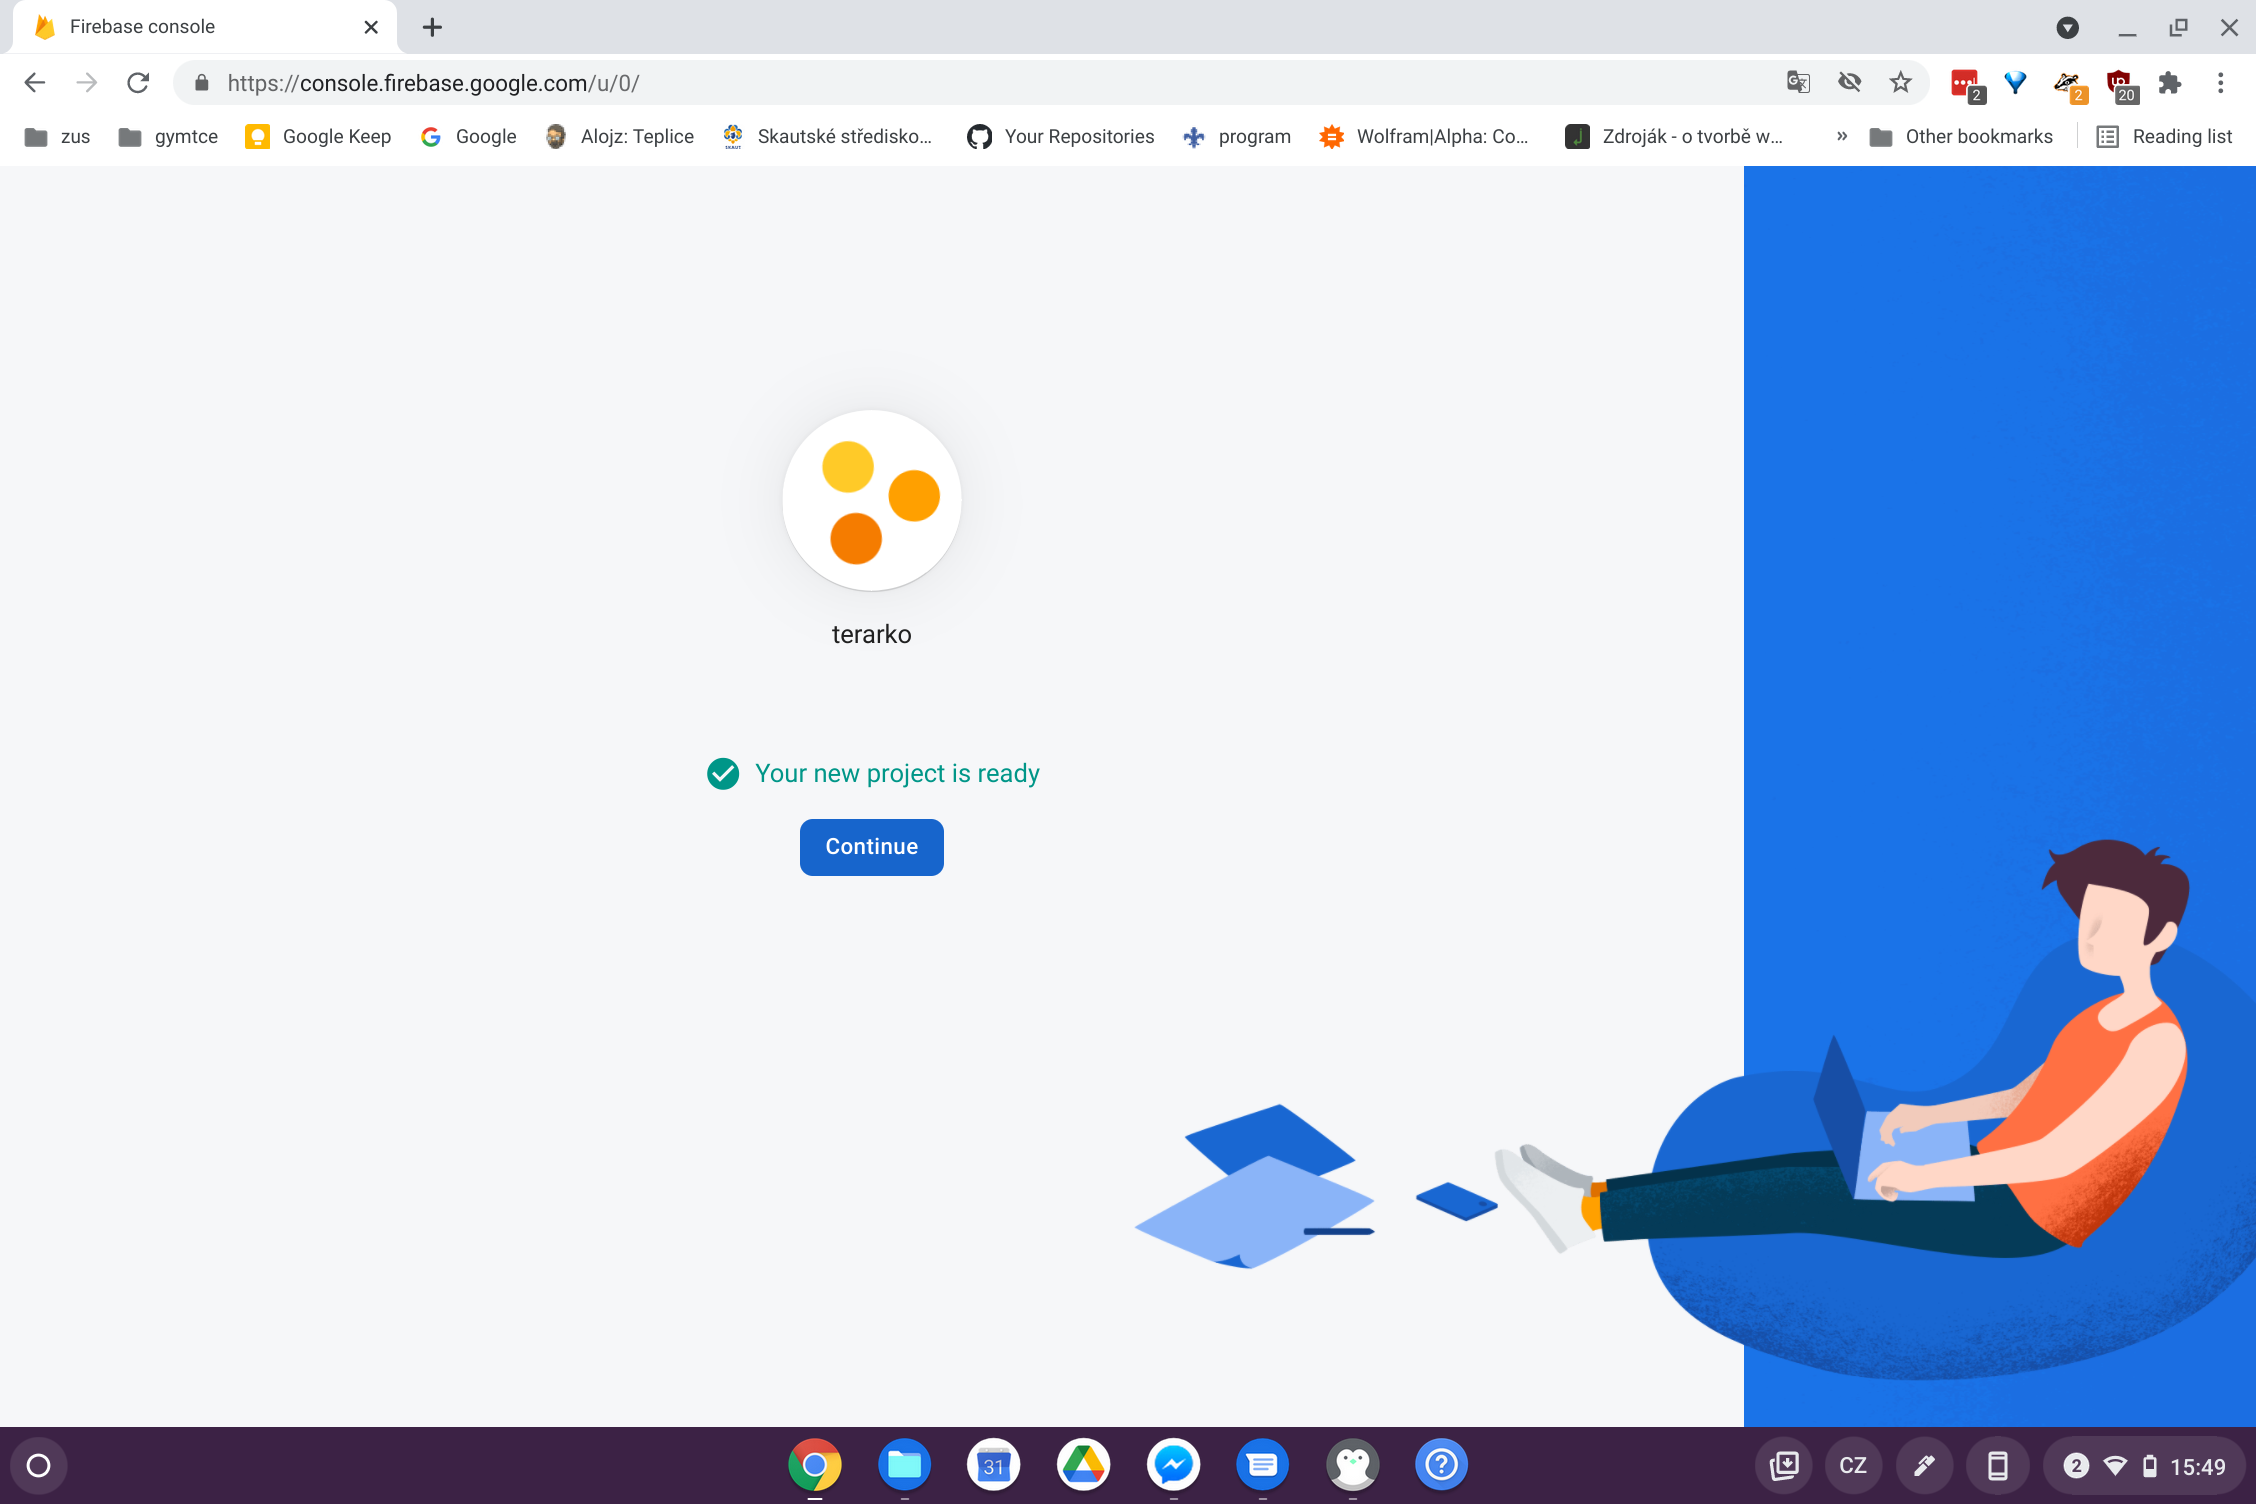
\includegraphics[width=0.8\textwidth]{firebase-fin.png}
    \caption{Firebase, hotovo}
\end{figure}
Vše jsem ponechal na výchozích hodnotách, teoreticky bych vzhledem k účelu mohl vypnout Google Analytics.
% dashboard
\begin{figure}[H]
    \centering
    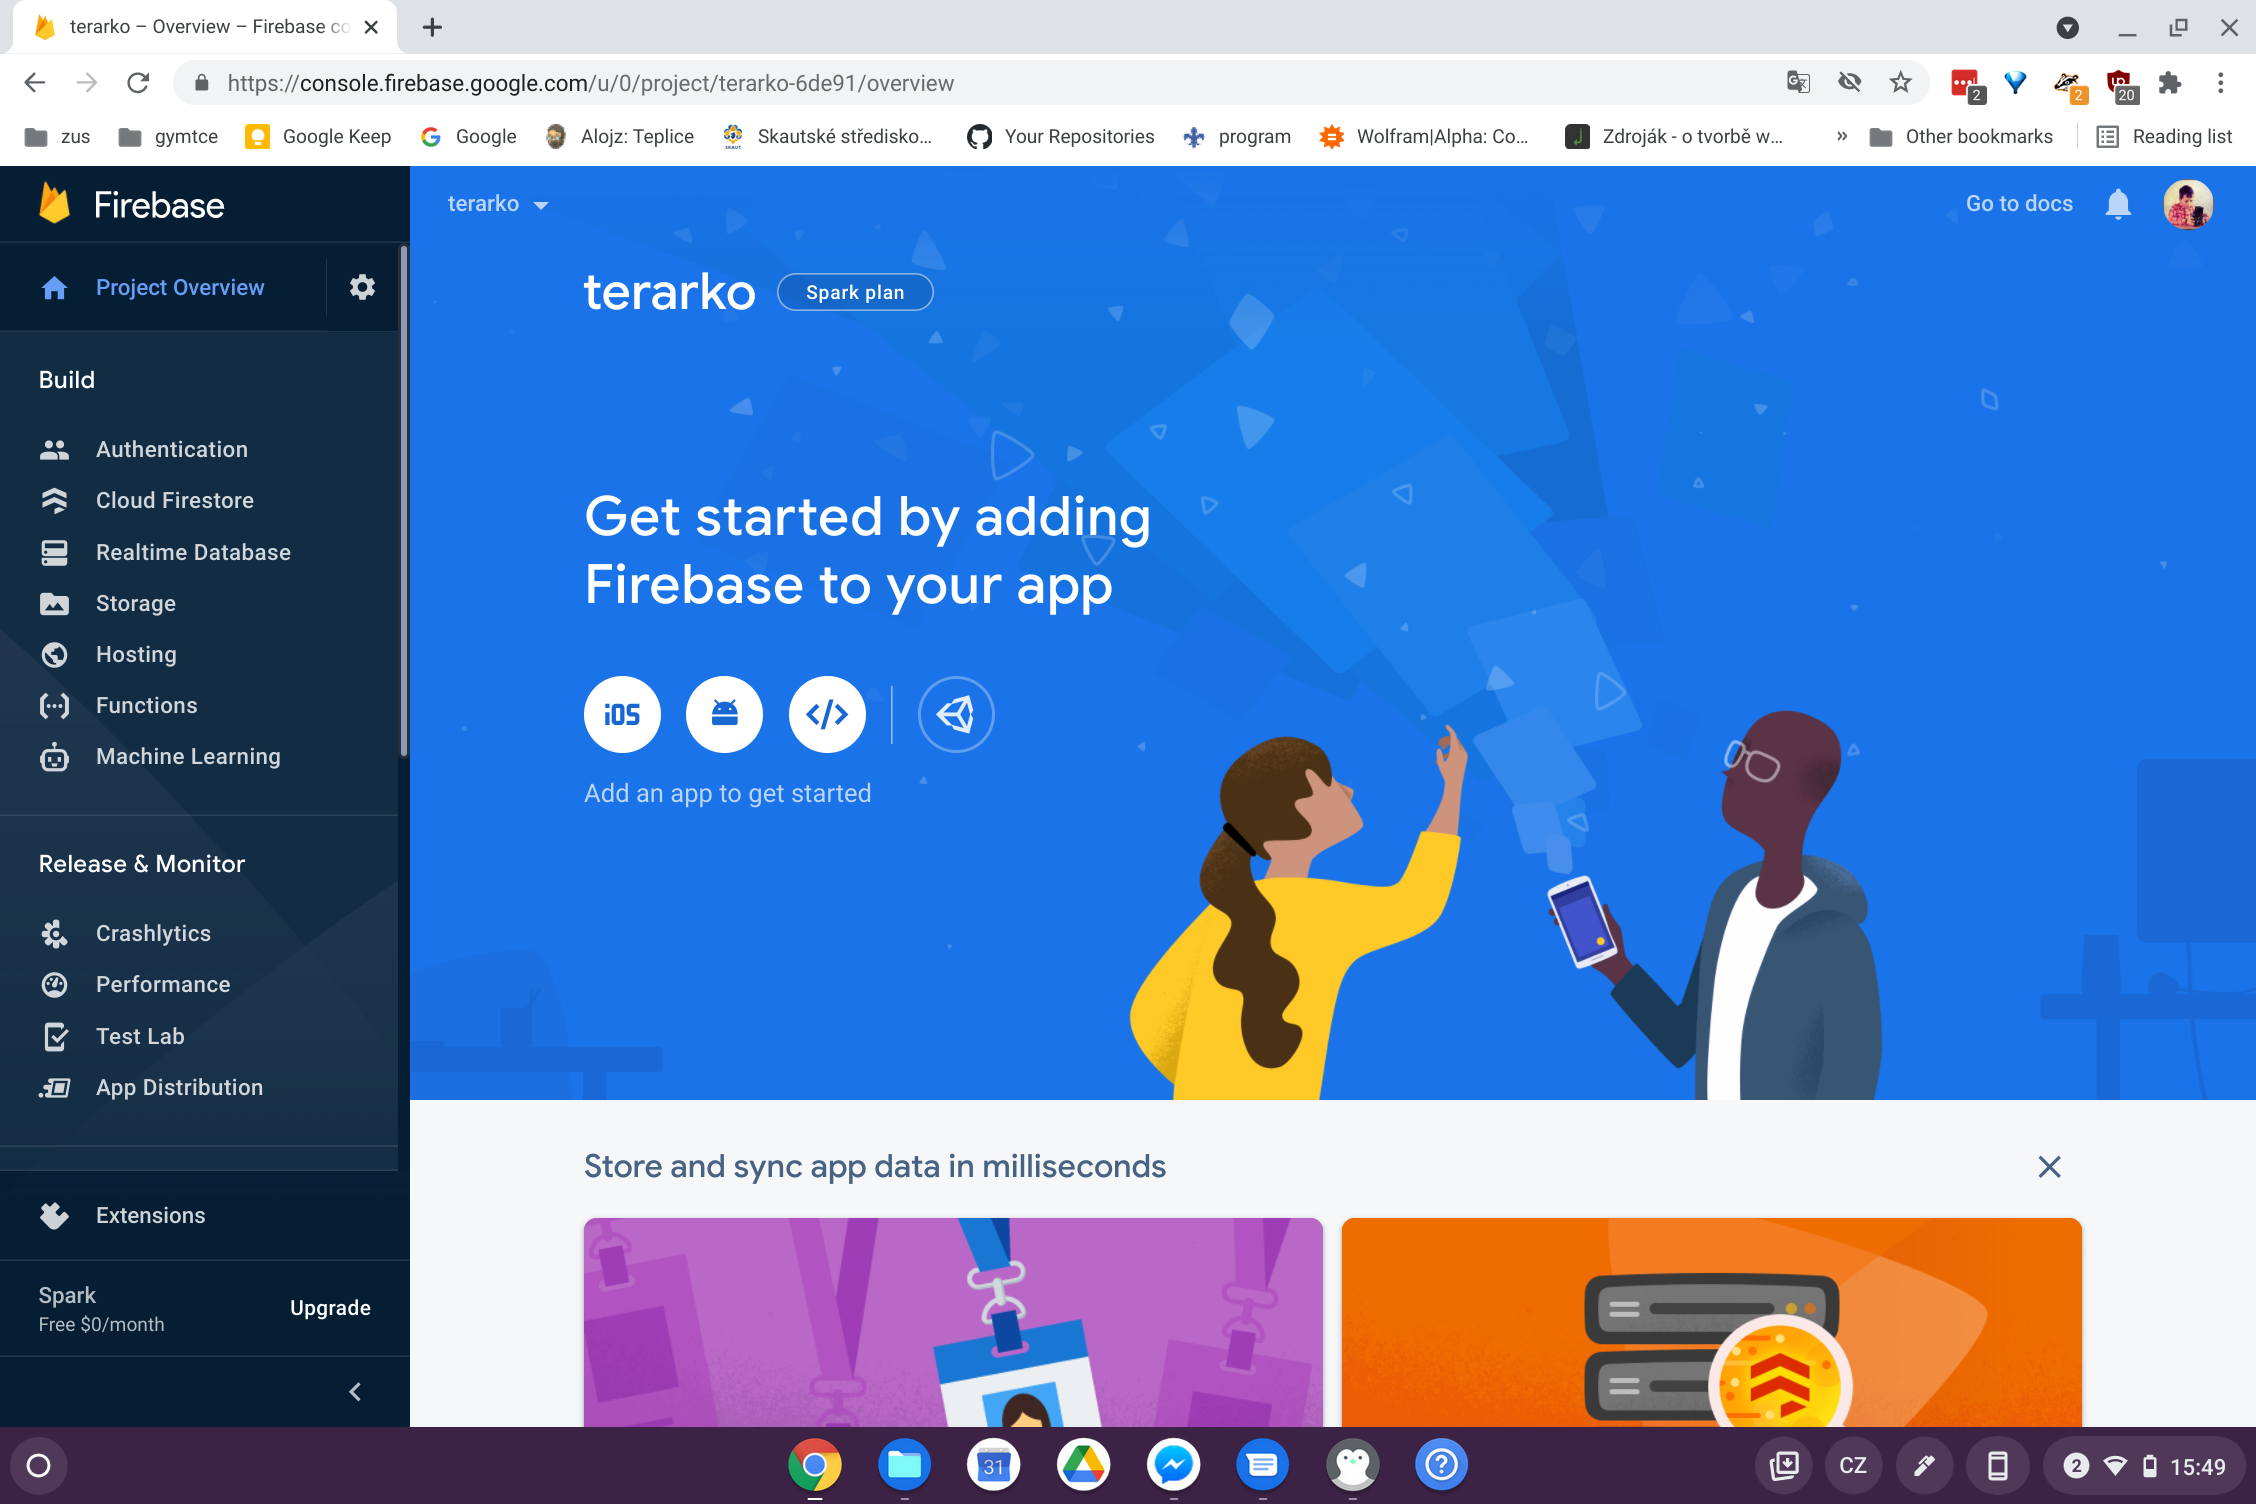
\includegraphics[width=0.8\textwidth]{firebase-dashboard.png}
    \caption{Firebase}
\end{figure}
Takto vypadá úvodní stránka \gls{firebase} po založení. Teď můžu přidat aplikace, které budu používat. Začnu firestorem, 
což je rychlá \gls{nosql} databáze, kterou budu používat pro ukládání naměřených hodnot. Opět se pokusím vysvětlit 
několika obrázky.

% krok 1
\begin{figure}[H]
    \centering
    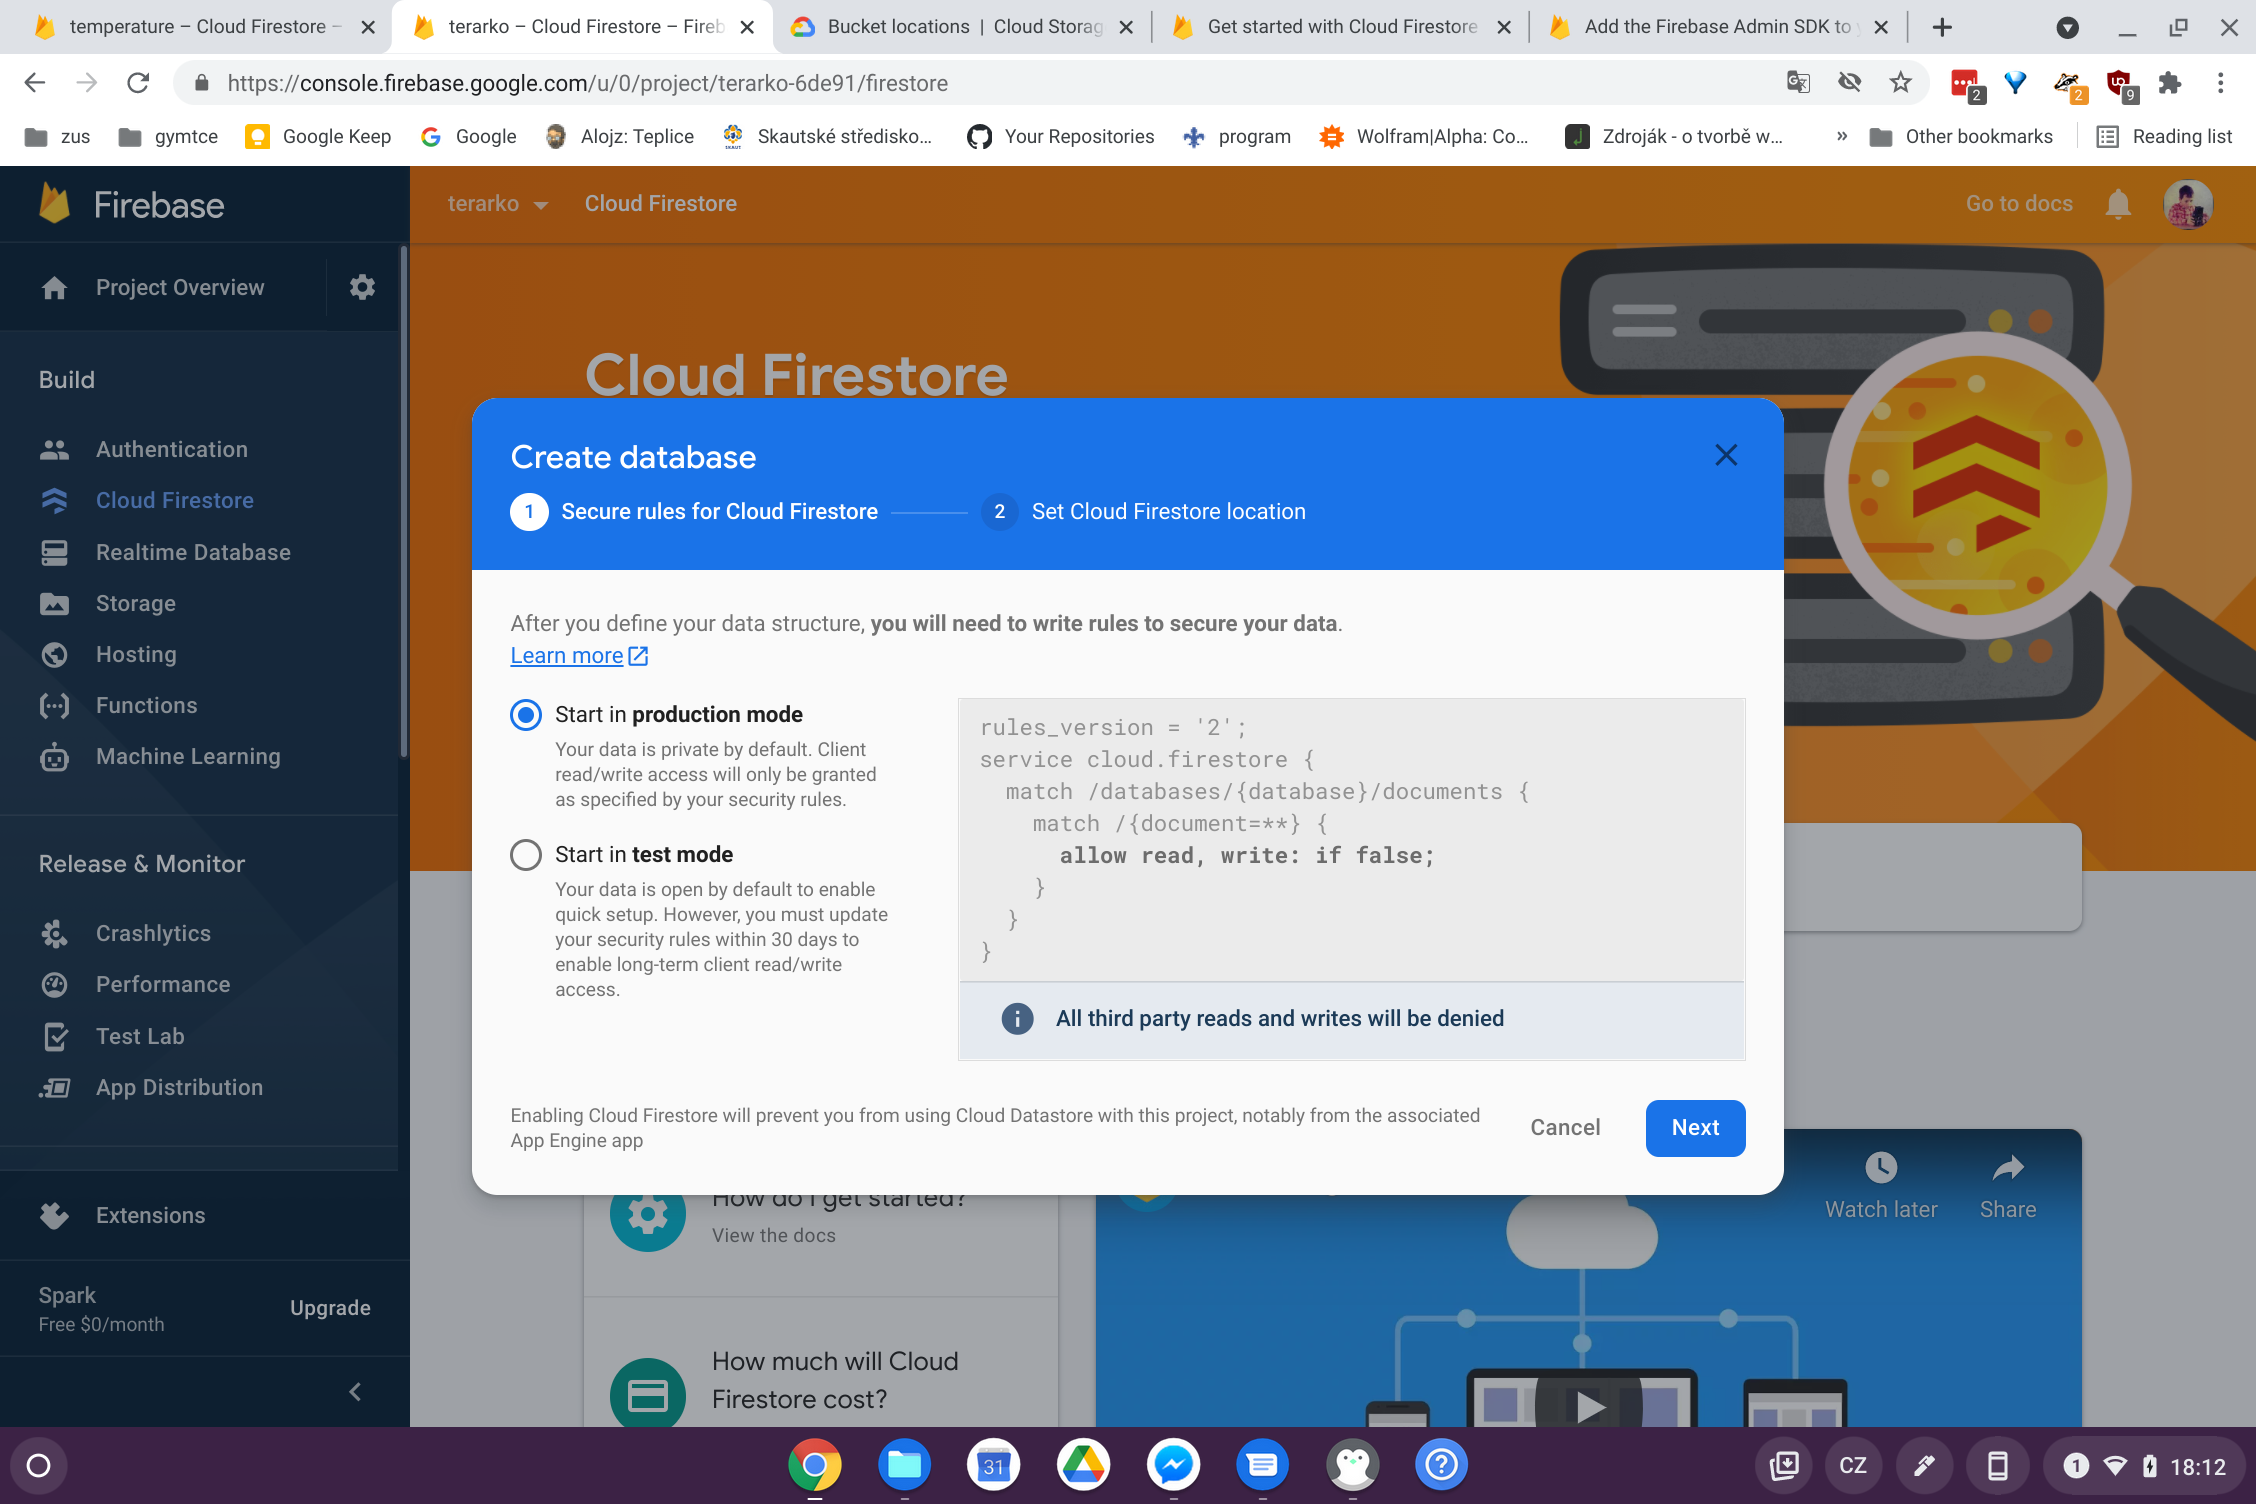
\includegraphics[width=0.8\textwidth]{firestore-1.png}
    \caption{Firestore, krok 1}
\end{figure}
Nastavení bezpečnosti použiji v produkčním módu, nechci aby se mi tam někdo připojoval bez přihlášení.
% krok 2
\begin{figure}[H]
    \centering
    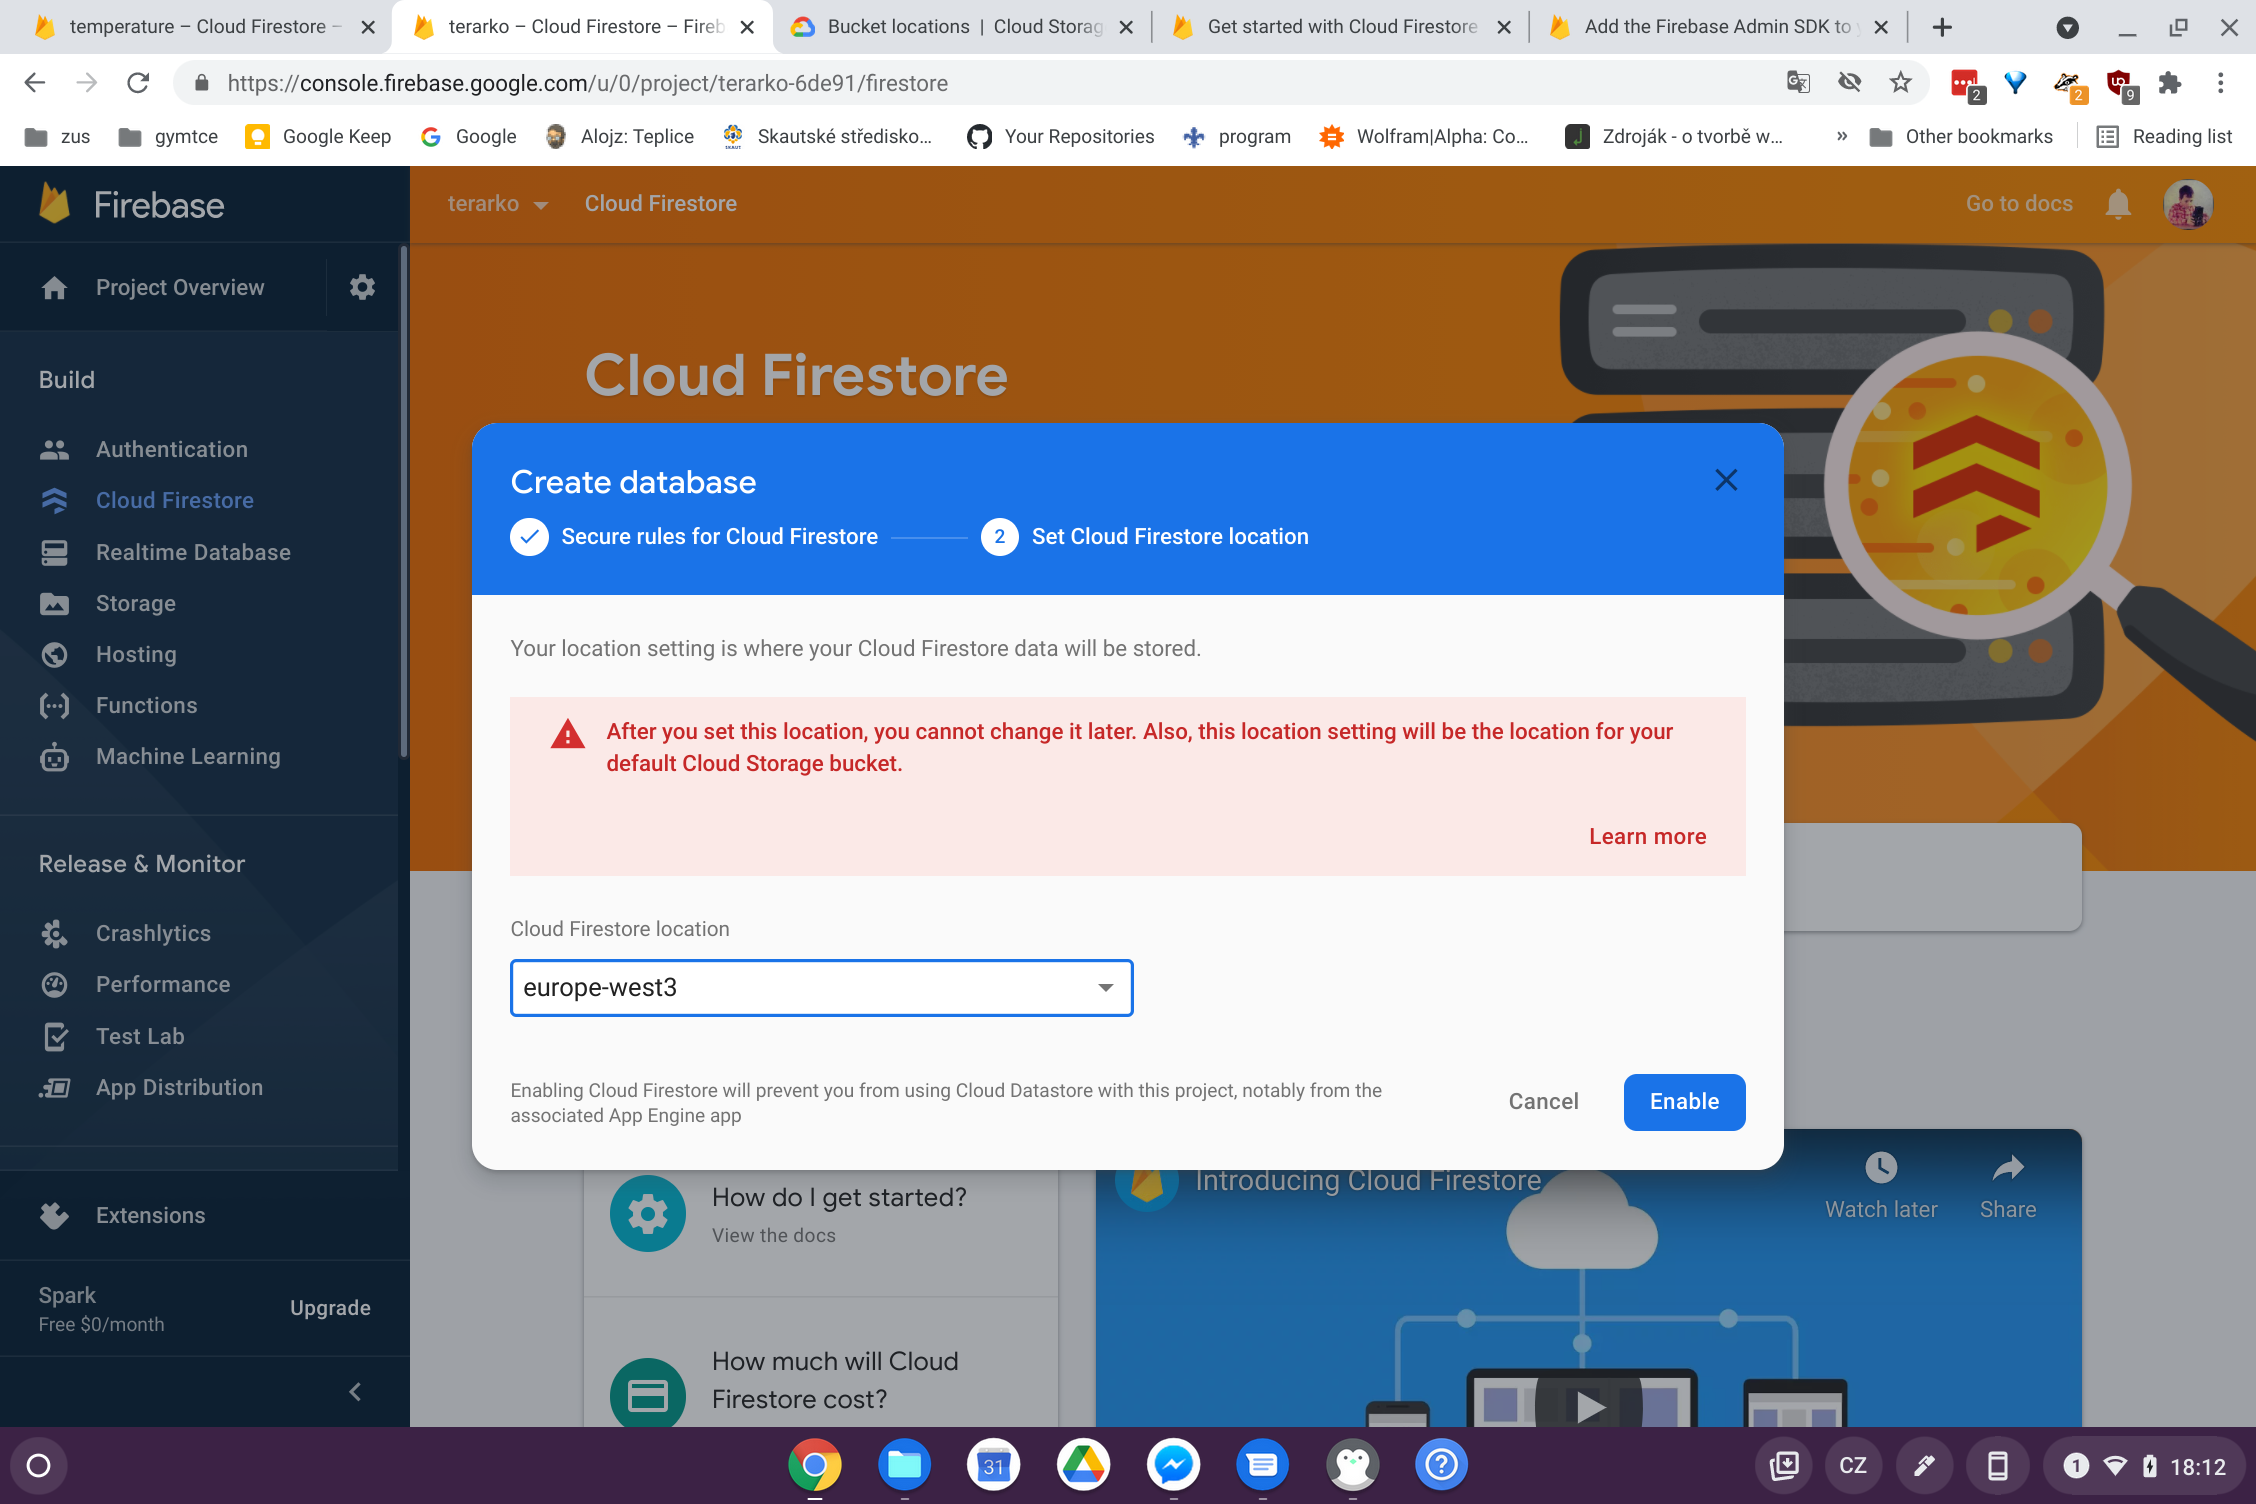
\includegraphics[width=0.8\textwidth]{firestore-2.png}
    \caption{Firestore, krok 2}
\end{figure}
Jako lokaci databáze volím Evropu konkrétně Frankfurt.
% dashboard
\begin{figure}[H]
    \centering
    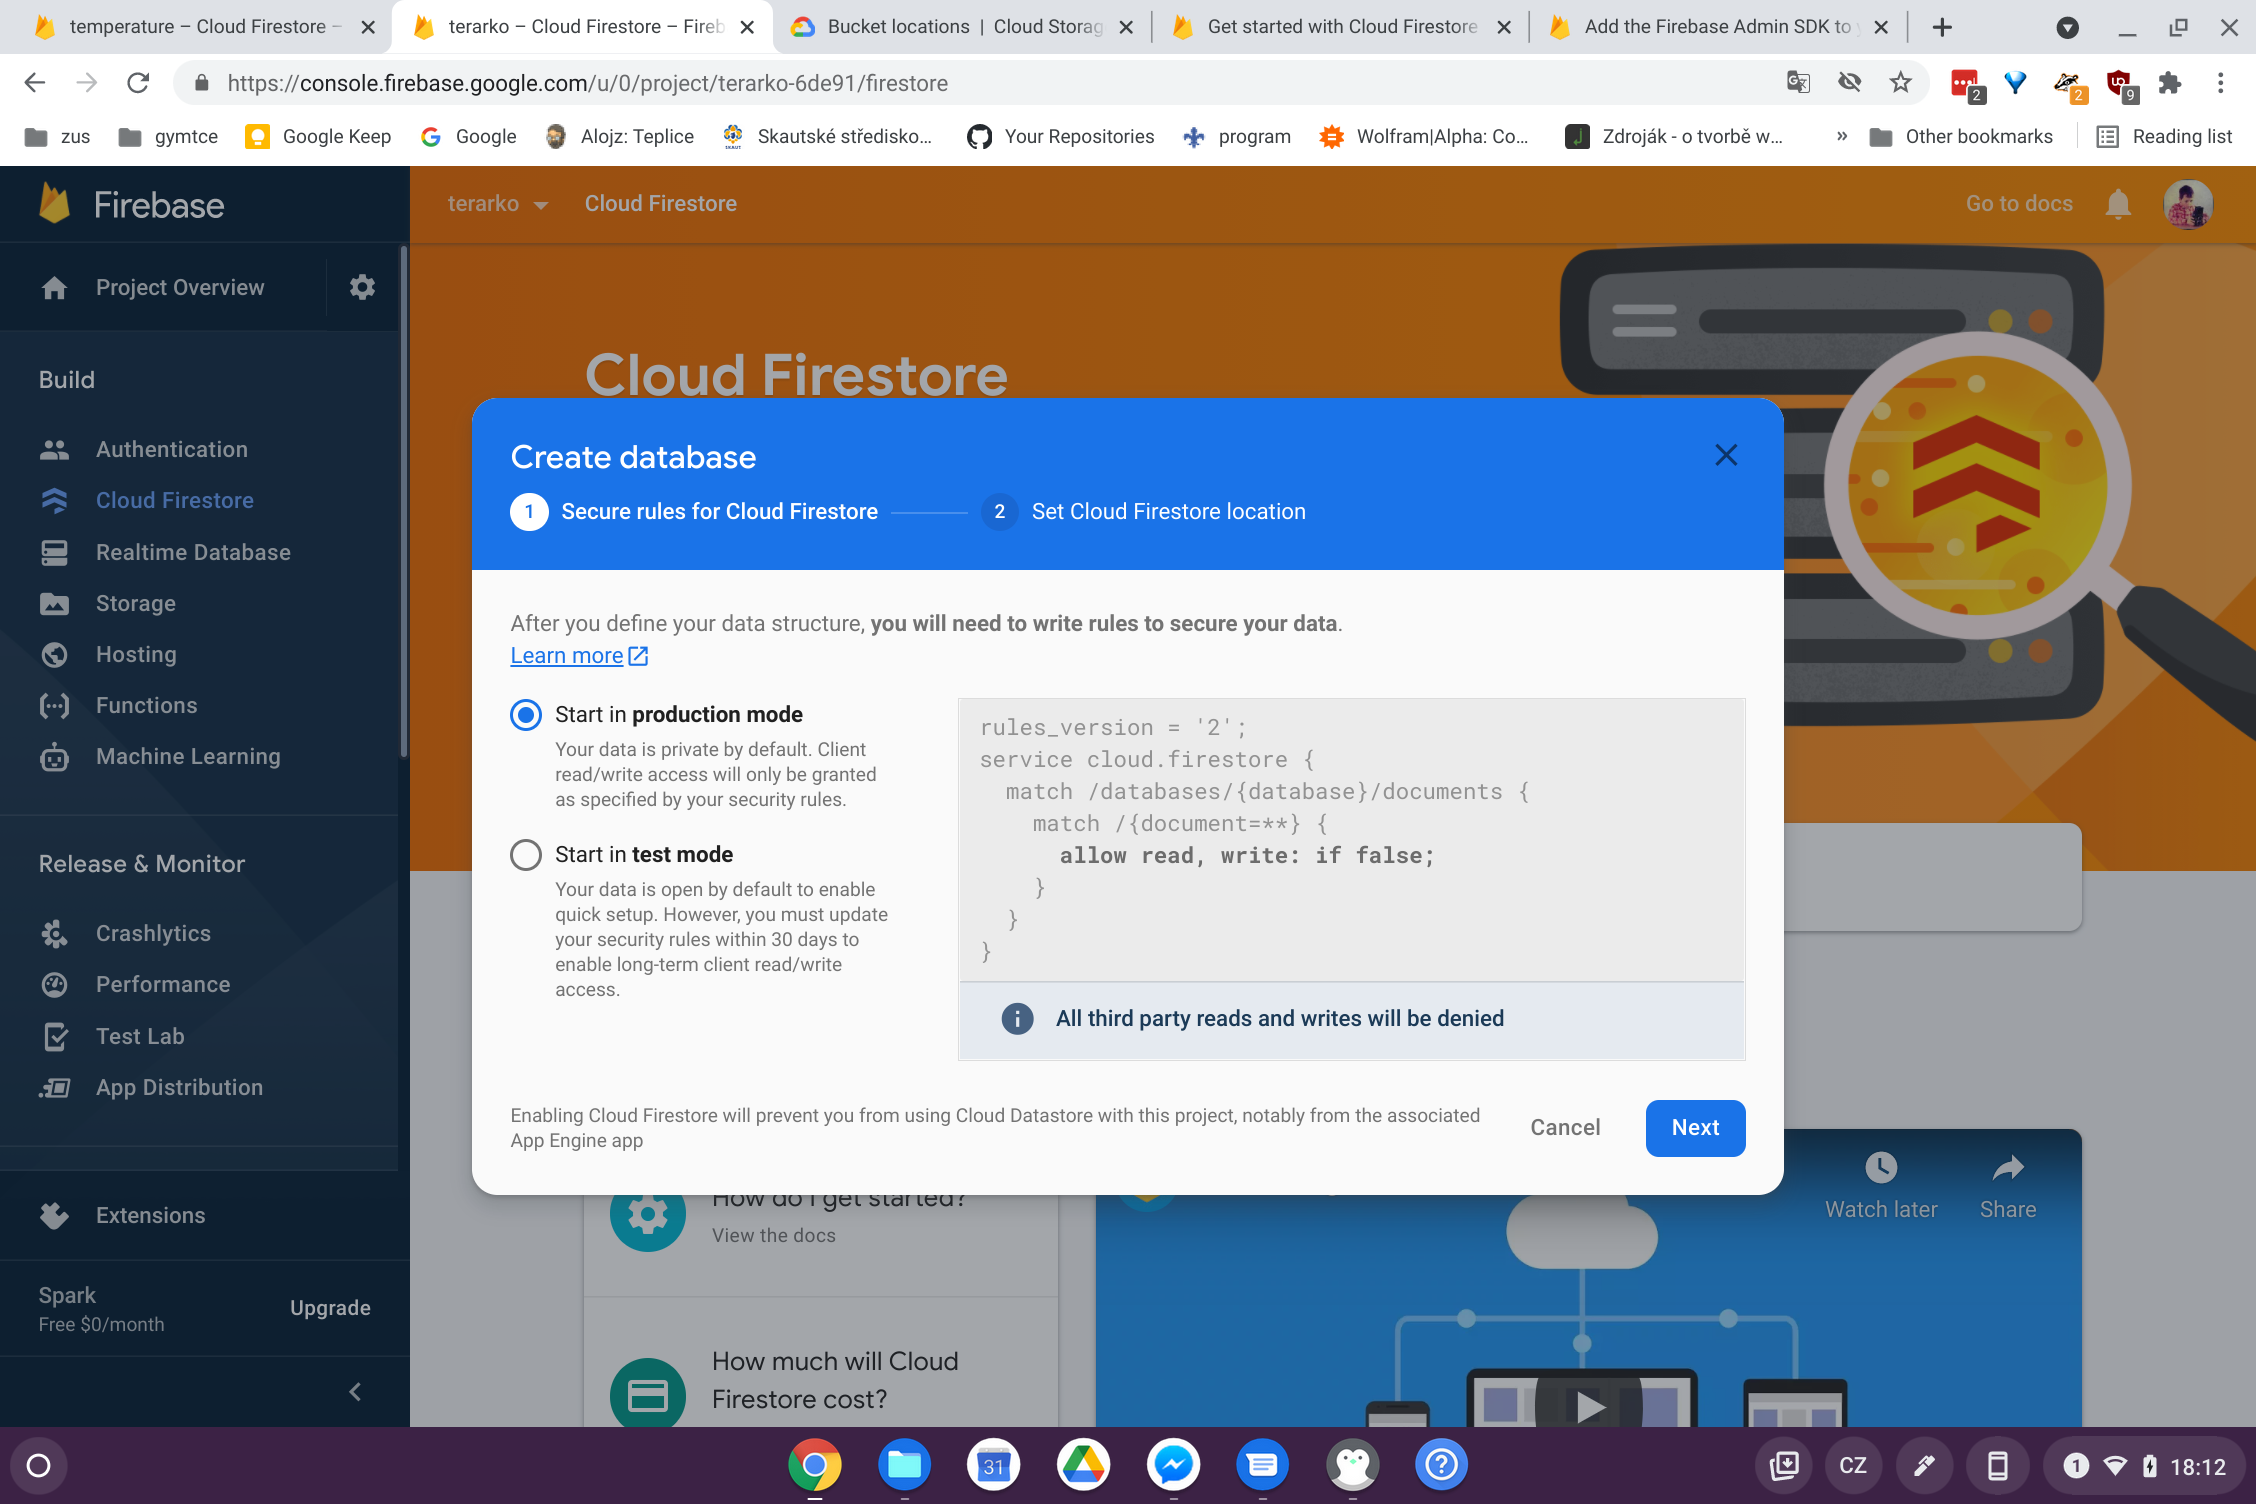
\includegraphics[width=0.8\textwidth]{firestore-1.png}
    \caption{Firestore, krok 1}
\end{figure}
A mám nastaveno. Teď můžu začít přidávat data.
